%----------------------------------------------------------------------------------------
%	PACKAGES AND DOCUMENT CONFIGURATIONS
%----------------------------------------------------------------------------------------
\documentclass[10pt,a4paper]{article}

\usepackage[utf8]{inputenc}
\usepackage[T1]{fontenc}
\usepackage[spanish]{babel}
\usepackage{amsmath}
\usepackage{amsfonts}
\usepackage{amssymb}
\usepackage{graphicx}
\usepackage{psfrag}
\usepackage{xcolor}
\usepackage{placeins}
\usepackage{enumerate}
\usepackage{tabularx}
\usepackage{tikz}
\usepackage{cite} % para contraer referencias
\usepackage[breaklinks=true]{hyperref}
\usepackage{titling}
\usepackage{caption}
\usepackage{float}
\restylefloat{table}


\graphicspath{ {images/} }

\usetikzlibrary{mindmap}
\pagestyle{empty}
%\usepackage[dvips]{graphicx}
\usepackage[left=2cm,right=2cm,top=2cm,bottom=2cm]{geometry}


\usepackage{color}
\definecolor{gray97}{gray}{.97}
\definecolor{gray75}{gray}{.75}
\definecolor{gray45}{gray}{.45}

\usepackage{listings}
\lstset{ frame=Ltb,
framerule=0pt,
aboveskip=0.5cm,
framextopmargin=3pt,
framexbottommargin=3pt,
framexleftmargin=0.4cm,
framesep=0pt,
rulesep=.4pt,
backgroundcolor=\color{gray97},
rulesepcolor=\color{black},
%
stringstyle=\ttfamily,
showstringspaces = false,
basicstyle=\small\ttfamily,
commentstyle=\color{gray45},
keywordstyle=\bfseries,
%
numbers=left,
numbersep=15pt,
numberstyle=\tiny,
numberfirstline = false,
breaklines=true,
}

% minimizar fragmentado de listados
\lstnewenvironment{listing}[1][]
{\lstset{#1}\pagebreak[0]}{\pagebreak[0]}

%%% Always I forget this so I created some aliases
\def\ContinueLineNumber{\lstset{firstnumber=last}}
\def\StartLineAt#1{\lstset{firstnumber=#1}}
\let\numberLineAt\StartLineAt


\lstdefinestyle{DOS}
{
  backgroundcolor=\color{black},
  basicstyle=\scriptsize\color{white}\ttfamily,
  columns=fullflexible,
  frame=single,
  breaklines=true,
  postbreak=\mbox{\textcolor{red}{$\hookrightarrow$}\space},
}

\lstdefinestyle{Java}
{language=Java,
}


%----------------------------------------------------------------------------------------
%	DOCUMENT INFORMATION
%----------------------------------------------------------------------------------------


\title{Práctica de Programación Orientada a Objetos – Curso 2022 / 2023
} % Title

\author{Angela Alexandra \textsc{Guzmán García} \\ \vspace{0.5em} \normalsize Correo electrónico: angelagn50@gmail.com
\vspace{0.5em} \normalsize Telefono: 642154124} % Nombre del autor y correo electrónico


\date{\today} % Date for the report

\begin{document}

\renewcommand{\listtablename}{Índice de tablas}
\renewcommand{\tablename}{Tabla}
\renewcommand{\lstlistingname}{Consola}

\maketitle % Insert the title, author and date

%----------------------------------------------------------------------------------------
%	SECTION
%----------------------------------------------------------------------------------------

\section{Decisiones de diseño:
}

La aplicación se desarrolló en tres momentos, inicialmente se realizó presenta a  través del planteamiento de la estructura de cada clase en lápiz y papel, así como  el  planteamiento del diagrama de casos de uso, de esta manera se generó una estructura inicial frente a la cual se busca dar respuesta a los planteamientos de la practica.
La aplicación está diseñada para que el programa siga ejecutándose y el usuario pueda navegar por el menú hasta que decida salir; en el método main el menú de opciones se implementó a través de un do-While el cual inicialmente da la bienvenida al usuario y propone 4 opciones de navegación, proveedor, cliente, administrados y salir de la aplicación, a medida que el usuario va eligiendo las opciones de menú y según el caso va avanzando por las diferentes tareas requeridas por la práctica en los tres puntos principales mostrando nuevamente el menú principal para evitar la terminación del programa hasta que el usuario así lo desee.

\subsection{Como usar la aplicación}



\begin{figure}[H]
  \centerline{
  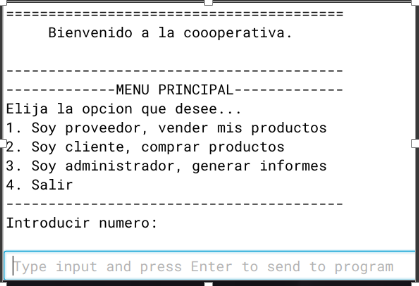
\includegraphics[width=10cm]{bienvenida.png}
  }
  \captionsetup{justification=centering}
  \caption{Menu bienvenido a la aplicación \label{fig:bienvenida} }
\end{figure}

El primer contacto de la aplicación con el usuario muestra un menú de bienvenida en el que se presentan 4 opciones según el usuario que se desee. Al introducir 1 se despliega la funcionalidad para el productor, la cual permite ingresar los productos que vayan a ser vendidos a la cooperativa.

\begin{figure}[H]
  \centerline{
  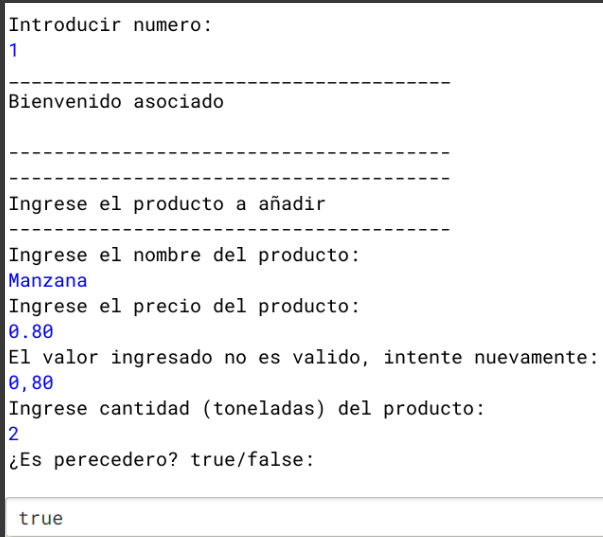
\includegraphics[width=8cm]{Opcion1MenuPrincipal.png}
  }
  \captionsetup{justification=centering}
  \caption{Ingresar producto \label{fig:opcion1MP} }
\end{figure}

En este ejemplo se agregan tres productos Manzana, Piña y Algodón.

\begin{figure}[H]
  \centerline{
  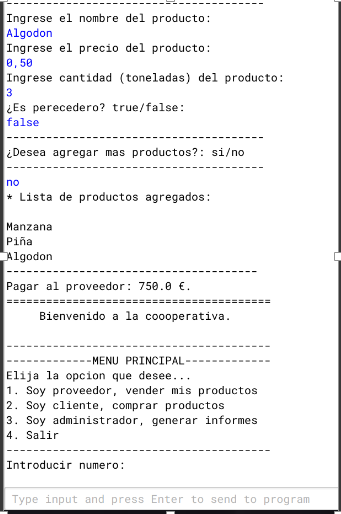
\includegraphics[width=8cm]{IngresoProducto.png}
  }
  \captionsetup{justification=centering}
  \caption{Lista de productos agregados y cantidad a pagar al proveedor \label{fig:opcionMP} }
\end{figure}

Como se observa en la imagen anterior, la aplicación ofrece  una lista de productos agregados y el valor neto a pagar al proveedor por parte de la cooperativa por sus productos. Y para evitar que el programa termine, se presenta nuevamente el menú principal para que el usuario explore las siguientes funcionalidades.

\begin{figure}[H]
  \centerline{
  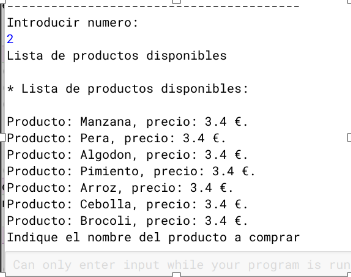
\includegraphics[width=8cm]{Opcion2MenuPrincipal.png}
  }
  \captionsetup{justification=centering}
  \caption{Ingresar producto \label{fig:opcion1MP} }
\end{figure}

La opción numero 2 del menú principal realiza las operaciones requeridas por los clientes a la hora de comprar productos, en este caso, se muestra una lista de productos disponibles, el usuario indica que producto o productos  quiere comprar de la lista y se crea una lista llamada cesta en la que se guardan los productos que el cliente ha elegido como se muestra a continuación.

\begin{figure}[H]
  \centerline{
  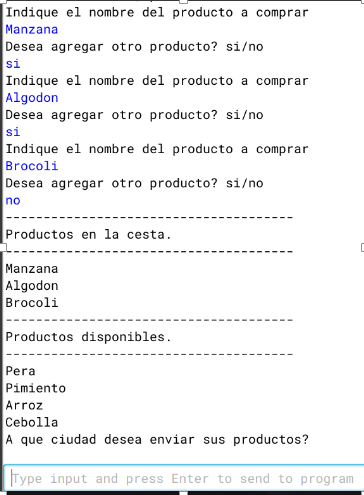
\includegraphics[width=8cm]{Cesta.png}
  }
  \captionsetup{justification=centering}
  \caption{Productos en cesta y disponibles \label{fig:opcion1MP} }
\end{figure}

De la misma manera, se presenta la lista de  productos disponibles que el cliente no ha elegido. Seguido a esto, se solicita el nombre de la ciudad a enviar el producto para gestionar la logística correspondiente.

\begin{figure}[H]
  \centerline{
  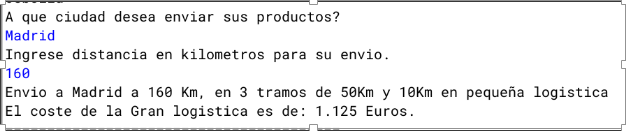
\includegraphics[width=12cm]{ciudad.png}
  }
  \captionsetup{justification=centering}
  \caption{Cálculo de tramos y precio de logistica \label{fig:opcion1MP} }
\end{figure}

La aplicación también pide al usuario la distancia para el envío y calcula los tramos a recorrer en gran logística y la distancia requerida en pequeña logística. Luego, calcula el coste de la gran logística y pequeña logística según la distancia, a continuación se muestra un ejemplo de cálculo en caso de que la distancia sea menor a 50 km lo que corresponde a pequeña logística.

\begin{figure}[H]
  \centerline{
  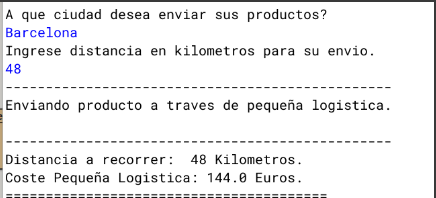
\includegraphics[width=8cm]{pLogistica.png}
  }
  \captionsetup{justification=centering}
  \caption{Calculo para envio de productos \label{fig:opcion1MP} }
\end{figure}



La opción 3 despliega un mensaje de bienvenido para el administrados y un menú de tres informes posibles a generar, de productos, de ventas y de rendimiento como se muestra a continuación.

\begin{figure}[H]
  \centerline{
  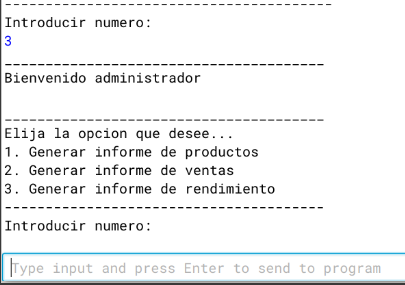
\includegraphics[width=8cm]{Informes.png}
  }
  \captionsetup{justification=centering}
  \caption{Menu informes \label{fig:opcion1MP} }
\end{figure}

Al elegir el informe de productos, la aplicación muestra un listado de productos y cantidad de ganancia por producto para el último año, como se muestra en la siguiente imagen.

\begin{figure}[H]
  \centerline{
  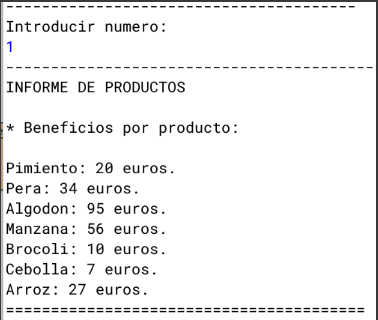
\includegraphics[width=8cm]{informeProductos.png}
  }
  \captionsetup{justification=centering}
  \caption{Informe de productos\label{fig:opcion1MP} }
\end{figure}

Para ir al siguiente informe, hay que pasar nuevamente por el menú principal y elegir la opción de administrador nuevamente
La opción informe de ventas muestra la cantidad de toneladas vendidas por producto en el último año.

\begin{figure}[H]
  \centerline{
  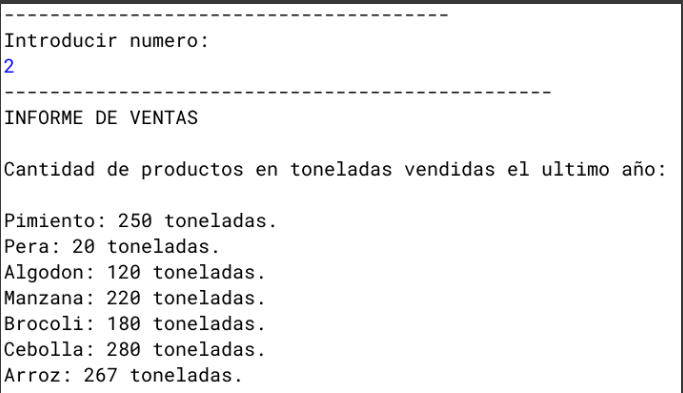
\includegraphics[width=10cm]{informeVentas.png}
  }
  \captionsetup{justification=centering}
  \caption{Ingresar ventas \label{fig:opcion1MP} }
\end{figure}

Para visualizar el informe de rendimiento, es necesario volver a ingresar la opción 3 en el menú principal y elegir el informe de rendimiento con la opción 3 nuevamente, la aplicación mostrará el informe de rendimiento el cual contiene el importe obtenido según productos, el importe obtenido según empresa de logística y el precio total de la logística en el último año.

\begin{figure}[H]
  \centerline{
  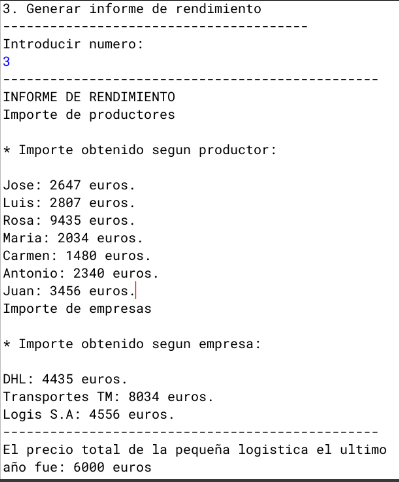
\includegraphics[width=8cm]{informeRendimiento.png}
  }
  \captionsetup{justification=centering}
  \caption{Ingresar producto \label{fig:opcion1MP} }
\end{figure}



%----------------------------------------------------------------------------------------
%	SECTION
%----------------------------------------------------------------------------------------

\section{Diagrama de clases}

Las clases PequenoProductor, GranProductor y ProductorFederado heredan de la clase Productor. Y de la misma manera, las clases PequenaLogistica y GranLogistica heredan de una clase padre llamada Logistica la cual a su vez hereda de una clase llamada Coste y ésta, a su vez hereda de la clase Producto.

También se han construido clases que enlazan el funcionamiento de la aplicación como la clase Pedido,  GestionPedidos y GestionProductos. Para el apartado 3 sobre informes, se han construido clases para cuatro tipos de informes las cuales son InformeEmpresa, InformeVentas, InformeProductor, InformeProductos.

La clase Cooperativa contiene el método main de la aplicación, para darle forma a la misma y para la interacción con el usuario se ha implementado una clase llamada imprimirMenu, la cual contiene las diferentes etapas de navegación del usuario por la aplicación.

\begin{figure}[H]
    \centering
    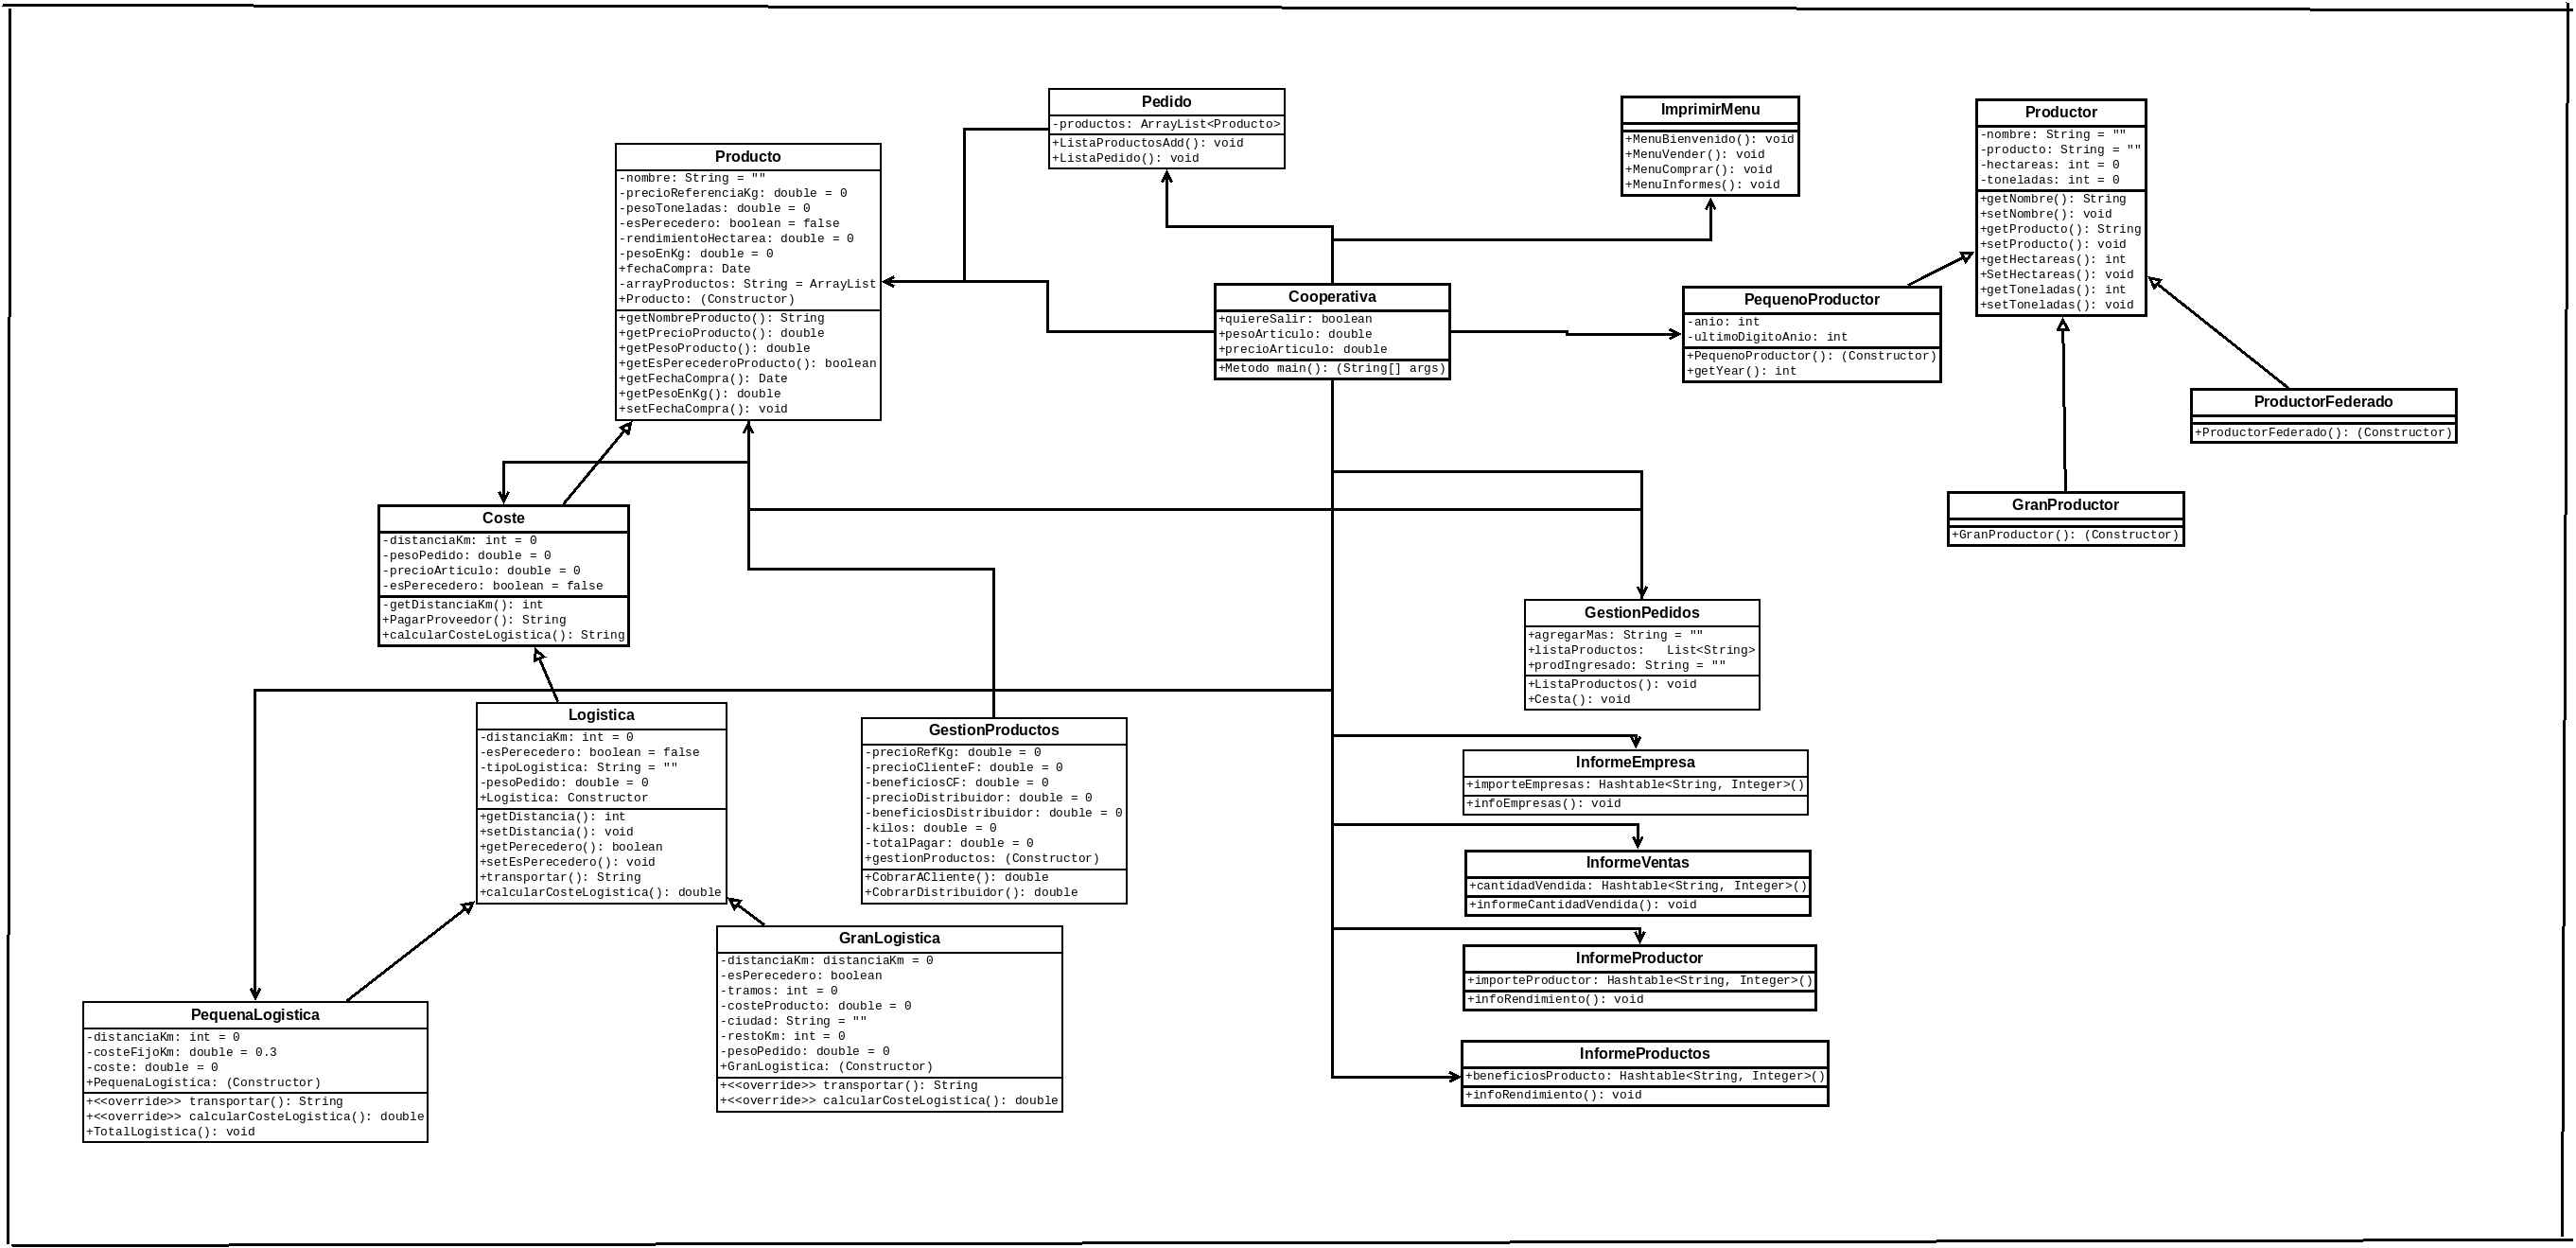
\includegraphics[width=\textwidth]{Diagrama_CoopEnBluej.png}
    \caption{Diagrama de clases}
    \label{fig:opcion1MP}
\end{figure}
  

%----------------------------------------------------------------------------------------
%	SECTION
%----------------------------------------------------------------------------------------

\section{Descripción de clases}

\StartLineAt{1}
\begin{lstlisting}[style=Java]
  import java.util.Scanner;
  import java.util.ArrayList;
  
  
  /**
   * Clase Cooperativa que contiene el metodo main y las acciones que realiza el usuario al interactuar con la aplicacion.
   * @author (Angela Alexandra Guzman Garcia) 
   * @version (001)
   */
  public class Cooperativa
  {
      public static void main(String[] args){
          //Declara variables
          boolean quiereSalir = false;
          double pesoArticulo = 0.5;
          double precioArticulo = 1.5; // Precio del articulo 
      
          do{
          ImprimirMenu menu = new ImprimirMenu();
          menu.MenuBienvenido();
          Scanner sc = new Scanner(System.in);
          System.out.println("Introducir numero: ");
          int opcion = sc.nextInt();
          
          switch(opcion){
              case 1:
                  menu.MenuVender();
                  
                  Pedido pedido1 = new Pedido(new ArrayList<Producto>()); // crea objeto de tipo Pedido
                  pedido1.ListaProductosAdd();
                  System.out.println("* Lista de productos agregados:\n");
                  pedido1.ListaPedido(); //Imprime la list
                  Coste costePedido = new Coste(); //Objeto tipo coste, parametro kilometros
                  
                  
                  String resultadoPago = costePedido.PagarProveedor(precioArticulo, pesoArticulo);
                  System.out.println("--------------------------------------");
                  System.out.println(resultadoPago); //Imprime el total en euros a pagar al proveedor
  
                  Coste pagar1 = new Coste();
                 
                  pagar1.PagarProveedor(precioArticulo, pesoArticulo);
                  break;
              case 2:
                  menu.MenuComprar();
                  sc.nextLine();
                  System.out.println("* Lista de productos disponibles:\n");
                  GestionPedidos pedido2 = new GestionPedidos(); //crea objeto de tipo GestionPedidos
                  pedido2.ListaProductos();
                  pedido2.Cesta();
                  
                  //Envia los productos 
                  //Pide por consola la ciudad y distancia en kilometros
                  System.out.println("A que ciudad desea enviar sus productos?");
                  String ciudad = sc.nextLine();
                  System.out.println("Ingrese distancia en kilometros para su envio.");
                  int km = sc.nextInt();
                  double costeProducto = 1.50;
                  PequenaLogistica pLogistica1 = new PequenaLogistica(km);
                  GranLogistica gLogistica1 = new GranLogistica(ciudad, km); //Crea objeto gran logistica
                  //Elige el tipo de logistica segun numero de kilometros
                  if(km <= 100){
                      System.out.println(pLogistica1.Transportar());
                      System.out.println(pLogistica1.calcularCosteLogistica());
                  }else{
                      System.out.println(gLogistica1.Transportar());
                      System.out.println(gLogistica1.calcularCosteLogistica(pesoArticulo, km, costeProducto));
                  }   
                  break;
              case 3:
                  // informes
                  menu.MenuInformes();
                  System.out.println("Introducir numero: ");
                  int opc = sc.nextInt();
                  switch(opc){
                      case 1:
                          //INFORME DE PRODUCTOS
                          System.out.println("------------------------------------------------");
                          System.out.println("INFORME DE PRODUCTOS \n     ");
                          PequenoProductor pProductor1 = new PequenoProductor("Pedro", "Platano", 3, 1);
                          pProductor1.MostrarPequeProductores();
                          //crea objeto para mostrar el informe de productos
                          InformeProductos informep = new InformeProductos();
                          informep.infoRendimiento();
                          break;
                      case 2:
                          //INFORME DE VENTAS
                          System.out.println("------------------------------------------------");
                          System.out.println("INFORME DE VENTAS \n     ");
                          InformeVentas informes = new InformeVentas();
                          informes.informeCantidadVendida();
                          break;
                          
                      case 3:
                          //INFORME DE RENDIMIENTO3
                          System.out.println("------------------------------------------------");
                          System.out.println("INFORME DE RENDIMIENTO ");
                          //crea un objeto y llama a sus metodos
                          InformeProductor informeR = new InformeProductor();
                          System.out.println("Importe de productores\n");
                          informeR.infoRendimiento();
                          InformeEmpresa informeE = new InformeEmpresa();
                          System.out.println("Importe de empresas\n");
                          informeE.infoEmpresas();
                          PequenaLogistica l1 = new PequenaLogistica(500);
                          l1.TotalLogistica();
                          break;
                  }
                  break;
              case 4:
                  quiereSalir = true;
                  System.out.println("Hasta Pronto");
                  break;
              default:
                  menu.MenuBienvenido();
                  break;
              }
      }while(quiereSalir != true);  
      }
  }
\end{lstlisting}

El programa se inicia en la clase Cooperativa, que contiene el método principal main y se encarga de interactuar con el usuario. A través de menús, el usuario puede realizar diferentes acciones.

El programa utiliza varias clases para representar diferentes conceptos. La clase ImprimirMenu se encarga de imprimir los menús en la consola para que el usuario pueda seleccionar una opción. La clase Pedido representa un pedido y contiene una lista de productos. La clase Coste gestiona los costos y pagos relacionados con los pedidos y proveedores.

La clase GestionPedidos se encarga de gestionar los pedidos de productos disponibles en la cooperativa. Permite al usuario ver la lista de productos y agregarlos a una cesta. Además, se utilizan las clases PequenaLogistica y GranLogistica para gestionar la logística de transporte, considerando distancias cortas y largas respectivamente.

También se incluyen clases como PequenoProductor que representan a los pequeños productores, y clases de informes como InformeProductos, InformeVentas, InformeProductor y InformeEmpresa, que generan informes relacionados con productos, ventas, rendimiento y empresas respectivamente.

En general, el programa permite al usuario realizar acciones como vender productos, realizar pedidos, calcular costos de logística, generar informes y más. Cada clase desempeña un papel específico en el funcionamiento del sistema de gestión de la cooperativa, interactuando entre sí para proporcionar las funcionalidades requeridas.

\StartLineAt{1}
\begin{lstlisting}[style=Java]
  import java.util.ArrayList;
  import java.util.Date;
  
  /**
   * Clase Producto gestiona los productos 
   * en la cooperativa.
   * @author (Angela Alexandra Guzman Garcia) 
   * @version (001)
   */
  public class Producto
  {
      // Declarar variables
      private String nombre;
      static double precioReferenciaKg;
      private double pesoToneladas;
      private boolean esPerecedero;
      private double pesoEnKg;
      public Date fechaCompra;
      
      private ArrayList<String> arrayProductos;
      
  
      /**
       * Constructor for objects of class Producto
       */
      public Producto(String nombreArticulo, double precioArticulo, 
                      double pesoArticulo, boolean esPerecederoArticulo )
      {
          // initialise instance variables
          this.nombre = nombreArticulo;
          this.precioReferenciaKg = precioArticulo;
          this.pesoToneladas = pesoArticulo;
          this.esPerecedero = esPerecederoArticulo;
      }
      public Producto(double precioArticulo, double pesoArticulo)
      {
          // initialise instance variables
          this.precioReferenciaKg = precioArticulo;
          this.pesoToneladas = pesoArticulo;
  
      }
  
      /**Metodos get
       */
      public String getNombreProducto()
      {
          return this.nombre;
      }
      public double getPrecioProducto()
      {
          return  this.precioReferenciaKg;
      }
      public double getPesoProducto()
      {
          return  this.pesoToneladas;
      }
       public boolean getEsPerecederoProducto()
      {
          return  this.esPerecedero;
      }
      public Date getFechaCompra(){
          return this.fechaCompra;
      }
      
      /**Metodos set
       */
      public void setFechaCompra(Date fechaCompra){
          this.fechaCompra = fechaCompra;
      }
      /**Convierte las toneladas a kilogramos
       */
  
      public double getPesoEnKg(){
          pesoEnKg = pesoToneladas * 1000;
          return this.pesoEnKg;
      }
      @Override
      public String toString(){
          return "Producto: " + nombre + ", precio: " + precioReferenciaKg;
      }  
  }
\end{lstlisting}

La clase Producto representa un artículo gestionado en la cooperativa. Tiene atributos como el nombre, precio de referencia por kilogramo, peso en toneladas, indicador de si es perecedero y la fecha de compra. También contiene una lista de productos representada por un ArrayList.

El constructor de la clase permite inicializar los atributos del producto. Se pueden proporcionar el nombre, precio, peso y si es perecedero. También hay un constructor adicional para casos donde solo se proporciona el precio y el peso.

La clase Producto proporciona métodos de acceso (get) para obtener el nombre, precio, peso y si es perecedero del producto. Además, hay un método getFechaCompra para obtener la fecha de compra.

La clase también incluye métodos de modificación (set) para establecer la fecha de compra.

El método getPesoEnKg convierte el peso en toneladas a kilogramos.

Además, se ha implementado el método toString para devolver una representación en cadena del producto, que incluye el nombre y el precio.

\StartLineAt{1}
\begin{lstlisting}[style=Java]

  
 public class Coste extends Producto {
 
     // variables de instancia
     private static int distanciaKm;
     private double pesoPedido;
     private double precioArticulo;
     private boolean esPerecedero;
   
     public Coste() {
         super("Arroz", distanciaKm, 0, true); // String double, double, boolean
         this.precioArticulo = precioArticulo;
         this.esPerecedero = esPerecedero;
         this.distanciaKm = distanciaKm;
         this.pesoPedido = pesoPedido;
     }
    
 
     public int getDistanciaKm() {
         return this.distanciaKm;
     }
 
     public String PagarProveedor(double precioArticulo, double pesoArticulo) {
 
         double tonelada = 1000;
         pesoPedido = (pesoArticulo * tonelada);
         double pagar = (precioArticulo * pesoPedido);
         String pagarString = Double.toString(pagar);
 
         return "Pagar al proveedor: " + pagarString;
     }
 
     public String calcularCosteLogistica() {
 
         return "Coste Logistica clase coste:";
     }
 
 }
 
\end{lstlisting}
La clase Coste hereda de la clase Producto y se encarga de calcular el costo a pagar al proveedor y el costo de la logística.

La clase contiene variables de instancia como la distancia en kilómetros, el peso del pedido, el precio del artículo y un indicador de si es perecedero.

El constructor de la clase inicializa los atributos con valores predeterminados, utilizando el constructor de la clase base (Producto) y asignando valores a las variables de instancia.

La clase proporciona un método getDistanciaKm para obtener la distancia en kilómetros.

La clase Coste se encarga de calcular los costos relacionados con el proveedor y la logística, utilizando información como la distancia, el peso y el precio del artículo. Hereda de la clase Producto y extiende su funcionalidad para proporcionar cálculos específicos de costos.

\StartLineAt{1}
\begin{lstlisting}[style=Java]
 
/**
* Clase Producto que contiene las caracteristicas necesarias de cada producto para que pueda ser gestionado en la cooperativa.
* 
* @author (Angela Alexandra Guzman Garcia) 
* @version (001)
*/
public class Logistica extends Coste
{
   // instance variables - replace the example below with your own
   private int distanciaKm;
   private  boolean esPerecedero;
   private double pesoPedido;
   public double precioArticulo;


   /**
    * Constructor for objects of class Logistica
    */
   public Logistica(int distanciaKm)
   {
       // inicializa variables de instancia
       super(); 
        this.distanciaKm = distanciaKm;
        this.esPerecedero = esPerecedero;
        this.pesoPedido = pesoPedido;
   }
   
    public int getDistancia()
   {
       return  this.distanciaKm;
   }
    public void setDistancia(int distanciaKm) {
       this.distanciaKm = distanciaKm;
   }
    public boolean getPerecedero()
   {
       return  this.esPerecedero;
       
   }
    public void setEsPerecedero(boolean esPerecedero) {
       this.esPerecedero = esPerecedero;
   }
   
    public String Transportar(){
        return "transportar de logistica";
   }
}
\end{lstlisting}

la clase Logistica se utiliza para gestionar la logística de un producto en la cooperativa. Hereda funcionalidad de la clase Coste y proporciona métodos y atributos específicos como la distancia, la perecibilidad y la acción de transportar.

La clase tiene variables de instancia como la distancia en kilómetros, un indicador de si el producto es perecedero, el peso del pedido y el precio del artículo. El constructor de la clase recibe la distancia en kilómetros y asigna los valores a las variables de instancia.

De la misma manera la clase proporciona métodos para obtener y establecer la distancia, y para obtener y establecer si el producto es perecederoy el método Transportar devuelve una cadena que indica la acción de transportar asociada a la logística.


\StartLineAt{1}
\begin{lstlisting}[style=Java]
  /**
  * Clase PequenaLogistica que hereda los metodos Transportar y calcularCosteLogistica de la 
  * clase logistica, aplica polimorfismosobreescribiendo los metodos para ajustar a las caracteristicas 
  * particulares de la gran logistica.
  * @author (Angela Alexandra Guzman Garcia) 
  * @version (001)
  */
 public class PequenaLogistica extends Logistica
 {
     // variables de instancia
        private int distanciaKm;
        private double costeFijoKm = 0.3; 
        private double coste;
    
     /** Constructor inicializa las variables
      */
     public PequenaLogistica( int distanciaKm)
     {
         // inicializa variables
        super(distanciaKm);
        this.distanciaKm = distanciaKm;
     }
     
     @Override
     public String Transportar(){
         if(distanciaKm <= 100 ){
             System.out.println("------------------------------------------------");
             System.out.println("Enviando producto a traves de pequenia logistica.");
             System.out.println("------------------------------------------------");
     }
     String distanciaString =Integer.toString(distanciaKm); 
         return "Distancia a recorrer:  " + distanciaString + " Kilometros.";
     }
     /**Se sobrescribe el metodo calcularCosteLogistica para ajustar a Gran Logistica
      */
     @Override
     public String calcularCosteLogistica(){
         costeFijoKm = 3;
         coste = costeFijoKm * distanciaKm; 
         return "Coste Pequenia Logistica: " + coste + " Euros.";
     }
     int totalPLogistica = 6000;
     public void TotalLogistica(){
         System.out.println("------------------------------------------------");
         System.out.println("El precio total de la pequenia logistica el ultimo anio fue);
     }
 }
 
\end{lstlisting}

la clase PequenaLogistica representa la logística de la cooperativa para distancias cortas. Aplica el polimorfismo al sobrescribir métodos de la clase base Logistica para adaptarlos a las características particulares de la pequeña logística. Proporciona métodos y atributos específicos relacionados con el cálculo de costes y el envío de productos a través de la pequeña logística.
El constructor de la clase recibe la distancia en kilómetros y asigna el valor a la variable de instancia correspondiente.

El método Transportar sobrescrito imprime un mensaje indicando que el producto se enviará a través de la pequeña logística. Luego devuelve una cadena que muestra la distancia a recorrer en kilómetros.

El método calcularCosteLogistica tambien sobrescrito establece el coste fijo por kilómetro para la pequeña logística y calcula el coste total basado en la distancia. Luego devuelve una cadena que muestra el coste de la pequeña logística.


\StartLineAt{1}
\begin{lstlisting}[style=Java]

  /**
  * Clase GranLogistica que contiene los metodos Transportar y
  * calcularCosteLogistica
  * sobreescritos con polimorfismo para ajustar a las caracteristicas
  * particulares
  * de la gran logistica
  * 
  * @author (Angela Alexandra Guzman Garcia)
  * @version (001)
  */
 public class GranLogistica extends Logistica // Hereda de la clase Logistica
 {
     // variables de instancia
     private int distanciaKm;
     private boolean esPerecedero;
     private int tramos;
     private double costeProducto;
     private String ciudad;
     private int restoKm;
     private double pesoPedido;
 
 
     /**
      * Constructor inicializa las variables
      */
     public GranLogistica(String ciudad, int distanciaKm) {
         // initialise instance variables
         super(distanciaKm);
         this.distanciaKm = distanciaKm;
         this.esPerecedero = getPerecedero();
         this.costeProducto = getPrecioProducto();
         this.ciudad = ciudad;
         this.pesoPedido = pesoPedido; 
 
     }
 
     /**
      * Se sobrescribe el metodo transportar para ajustar a Gran Logistica
      */
     @Override
     public String Transportar() {
         tramos = distanciaKm / 50;
         restoKm = distanciaKm % 50;
         if (esPerecedero == true && distanciaKm > 100) {
             System.out.println("------------------------------------------------");
             System.out.println("Enviando producto a " + ciudad + ".\n");
             System.out.println("------------------------------------------------");
             System.out.println(
                     "Distancia a recorrer gran logistica:  " + distanciaKm + "Km, en " + tramos + " tramos de 50Km.");
             System.out.println("Distancia a recorrer pequenia logistica:  " + restoKm + "Km.");
         }
         return "Envio a "+ ciudad + " a " + distanciaKm + " Km, en " + tramos + " tramos de 50Km y " + restoKm
                 + "Km en pequenia logistica";
     }
 
     /**
      * Se sobrescribe el metodo calcularCosteLogistica para ajustar a Gran Logistica
      */
     // @Override
     public String calcularCosteLogistica(double pesoArticulo, int distanciaKm, double costeProducto) {
         int tramos = (distanciaKm / 50);
         double costeTotal = 0;
         for (int i = 0; i < tramos; i++) {
             double costeTramo = 0.5 * costeProducto * pesoArticulo;
             costeTotal += costeTramo;
         }
         String costeString = Double.toString(costeTotal);
         return "El coste de la Gran logistica es de: " + costeString + " Euros.";
     }  
 }
  
\end{lstlisting}

la clase GranLogistica representa la logística de la cooperativa para distancias largas. Utiliza la herencia y el polimorfismo para ajustar los métodos de la clase base Logistica a las características específicas de la gran logística. Proporciona métodos y atributos relacionados con el cálculo de costes, la distribución de kilómetros y el envío de productos a través de la gran logística.

El constructor de la clase recibe la ciudad y la distancia en kilómetros, y asigna los valores correspondientes a las variables de instancia.

El método Transportar sobrescrito calcula el número de tramos de 50 kilómetros y el resto de kilómetros que se enviarán a través de la pequeña logística. Si el producto es perecedero y la distancia es mayor a 100 kilómetros, muestra un mensaje indicando la ciudad de destino y la distancia a recorrer tanto en la gran logística como en la pequeña logística. Luego devuelve una cadena que indica el envío a la ciudad y la distribución de los kilómetros.

El método calcularCosteLogistica sobrescrito calcula el coste total de la gran logística basado en el peso del artículo, la distancia en kilómetros y el coste del producto. Divide la distancia en tramos de 50 kilómetros y calcula el coste de cada tramo. Luego devuelve una cadena que muestra el coste total de la gran logística.

\StartLineAt{1}
\begin{lstlisting}[style=Java]
  
/**
* Clase GestionProductos que realiza las acciones de calcular los importes a cada tipo de cliente.
* @author (Angela Alexandra Guzman Garcia) 
* @version (001)
*/
public class GestionProductos 
{
   // variables de instancia
   private double precioRefKg;
   private double precioClienteF;
   private double beneficiosCF;
   private double precioDistribuidor;
   private double beneficiosDistribuidor;
   private double kilos;
   private double totalPagar;
 

   /**
    * Constructor para objetos de la clase GestionProductos
    */
   public GestionProductos()
   {
       // inicializacion de variables de constructor
      
      Producto miProducto = new Producto ("Nombre producto", precioRefKg , 0.0, false);
      this.precioRefKg = miProducto.getPrecioProducto();
      this.kilos = miProducto.getPesoEnKg();
      
       
   }

   /** Funcion que aumenta el 15% al precio del cliente final segun el precio de referencia por kilogramo del producto
    */
   public double CobrarACliente(double precioRefKg)
   {
       // put your code here
       beneficiosCF = precioRefKg * 15 / 100;
       precioClienteF = precioRefKg + beneficiosCF;
       return precioClienteF;
   }
   
   /** Funcion que aumenta el 5% al precio del distribuidor segun el precio de referencia del producto
    */
   public double CobrarDistribuidor(double precioRefKg)
   {
      
       beneficiosDistribuidor = precioRefKg * 5 / 100;
       precioDistribuidor = precioRefKg + beneficiosDistribuidor;
       return precioDistribuidor;
   }
}

  
\end{lstlisting}

La clase GestionProductos se encarga de realizar acciones relacionadas con el cálculo de importes para diferentes tipos de clientes. Tiene variables de instancia que almacenan precios, beneficios y cantidades de productos. El constructor inicializa estas variables a través de la creación de un objeto de la clase Producto.


\StartLineAt{1}
\begin{lstlisting}[style=Java]
  import java.util.List;
  import java.util.ArrayList;
  import java.util.Scanner;
  
  /**
   * Clase GestionPedidos gestiona los productos 
   * disponibles en la cooperativa para comprar.
   * @author (Angela Alexandra Guzman Garcia) 
   * @version (001)
   */
  public class GestionPedidos
  {
          /**El metodo ListaProductos, crea elementos tipo Producto y luego los 
           * agrega a una lista, para finalmente mostrar la lista al usuario.
           */
          String agregarMas = "";
          String prodIngresado = "";
          //Declara una lista de productos
          List<Producto> listaProductos = new ArrayList<>();
          //Crea nueva lista de productos ingresados por el usuario.
          List<String> listCesta = new ArrayList<>();
          
      public void ListaProductos(){
          //Crea elementos tipo Producto
          Producto manzana = new Producto("Manzana", 3.4, 2, true);
          Producto pera = new Producto("Pera", 2.1, 1.5, true);
          Producto algodon = new Producto("Algodon", 4.3, 6, false);
          Producto pimiento = new Producto("Pimiento", 2.2, 3, true);
          Producto arroz = new Producto("Arroz", 1.4, 2.2, true);
          Producto cebolla = new Producto("Cebolla", 2.4, 2.6, true);
          Producto brocoli = new Producto("Brocoli", 1.4, 2.5, true);
  
          //agrega elementos a la lista
          listaProductos.add(manzana);
          listaProductos.add(pera);
          listaProductos.add(algodon);
          listaProductos.add(pimiento);
          listaProductos.add(arroz);
          listaProductos.add(cebolla);
          listaProductos.add(brocoli);
          
          //Imprime la lista de productos disponibles
          for(Producto producto : listaProductos){
              System.out.println(producto.toString());
          }   
      }   
      public void Cesta(){
          do{
              Scanner sc = new Scanner(System.in);
              System.out.println("Indique el nombre del producto a comprar");
              //Lee el producto aniadido por consola a la cesta
              String prodIngresado = sc.nextLine();
              //Aniade el producto a la cesta
              System.out.println("Desea agregar otro producto? si/no");
              agregarMas = sc.nextLine();
              //Verifica que la respuesta sea correcta
              while(!agregarMas.equals("si") && !agregarMas.equals("no")){
                  System.out.println("Valor no valido, intente nuevamente: ");
                  agregarMas = sc.nextLine();
              }
              
              listCesta.add(prodIngresado);
              //Recorre la lista y verifica que el producto ingresado este en la lista para luego removerlo
              for (int i= 0; i < listaProductos.size(); i++){
                  if(listaProductos.get(i).getNombreProducto().equalsIgnoreCase(prodIngresado)){
                      listaProductos.remove(i);
                      break;
                  }
              }
          }while(!agregarMas.equals("no")) ;
          //Imprime los productos de la cesta
          System.out.println("--------------------------------------");
          System.out.println("Productos en la cesta.");
          System.out.println("--------------------------------------");
          for(String producto : listCesta){
              System.out.println(producto);
          } 
          //Imprime de nuevo los productos disponibles 
          System.out.println("--------------------------------------");
          System.out.println("Productos disponibles.");
          System.out.println("--------------------------------------");
          for(int i = 0; i < listaProductos.size(); i++){
              System.out.println(listaProductos.get(i).getNombreProducto());
          }
      }
  }
  
\end{lstlisting}

La clase GestionPedidos se encarga de gestionar los productos disponibles en la cooperativa para su compra. Tiene dos métodos principales: ListaProductos y Cesta.

El método ListaProductos crea varios objetos de la clase Producto con diferentes características y los agrega a una lista llamada listaProductos. Luego, muestra por consola la lista de productos disponibles.

El método Cesta permite al usuario agregar productos a su cesta de compra. Solicita al usuario el nombre del producto a comprar, verifica si desea agregar más productos y registra los productos ingresados en una lista llamada listCesta. También elimina los productos seleccionados de la lista de productos disponibles. Finalmente, muestra por consola los productos en la cesta y los productos disponibles actualizados.

\StartLineAt{1}
\begin{lstlisting}[style=Java]
  import java.util.ArrayList;
  import java.util.Scanner;
  
  /**
   * Clase Pedido que pide al proveedor que ingrese los productos 
   * y los pone en una cesta de productos seleccionados.
   * @author (Angela Alexandra Guzman Garcia) 
   * @version (001)
   */
  public class Pedido
  {
      //Crea un array de productos tipo producto
      private ArrayList<Producto> listaProductos;
      //Declara el constructor
      public Pedido(ArrayList<Producto> listaProductos)
      {
          this.listaProductos = listaProductos;
          
      }
      
  
      //Metodo que agregados un producto a la lista
      public void ListaProductosAdd(){
          Scanner sc = new Scanner(System.in);
          String agregar = "si";
          
          do{
              System.out.println("---------------------------------------");
              System.out.println("Ingrese el producto a agregar");
              System.out.println("---------------------------------------");
              
              System.out.println("Ingrese el nombre del producto: ");
              String nombre = sc.nextLine();
              System.out.println("Ingrese el precio del producto: ");
              while(!sc.hasNextDouble()){
                  System.out.println("El valor ingresado no es valido, intente nuevamente: ");
                  sc.next();
              }
              double precio = sc.nextDouble();
              System.out.println("Ingrese cantidad (toneladas) del producto: ");
              double cantidad = sc.nextDouble();
              System.out.println("Es perecedero truefalse:");
              boolean perecedero = sc.nextBoolean();
              System.out.println("---------------------------------------");
              System.out.println("Desea agregar mas productos: si/no");
              System.out.println("---------------------------------------");
              String teclado = sc.nextLine();
              
              Producto producto1 = new Producto(nombre, precio, cantidad, perecedero);
              this.listaProductos.add(producto1);
              
              agregar = sc.nextLine();
          }while(agregar.equalsIgnoreCase("si"));
          
      }
      
       public void ListaPedido(){
      for (Producto producto : listaProductos){
          System.out.println(producto.getNombreProducto());
      }
      }
  }
\end{lstlisting}


La clase Pedido se utiliza para solicitar al proveedor que ingrese los productos y almacenarlos en una lista de productos seleccionados. Tiene dos métodos principales: ListaProductosAdd y ListaPedido.

El método ListaProductosAdd permite al proveedor ingresar los detalles de un producto, como el nombre, el precio, la cantidad y si es perecedero. Luego, crea un objeto de la clase Producto con los detalles ingresados y lo agrega a la lista listaProductos. El proveedor puede continuar ingresando más productos hasta que decida no agregar más.

El método ListaPedido muestra por consola los nombres de los productos almacenados en la lista listaProductos.

\StartLineAt{1}
\begin{lstlisting}[style=Java]

  /**
  * Clase Productor, contiene los detalles de cada producto y los metodos set y get.
  * @author (Angela Alexandra Guzman Garcia) 
  * @version (001)
  */
 public class Productor
 {
     // Variables
     private String nombre;
     private String producto;
     private int hectareas;
     private int toneladas;
     
     public Productor(String nombre, String producto, int hectareas, int toneladas) {
         this.nombre = nombre;
         this.producto = producto;
         this.hectareas = hectareas;
         this.toneladas = toneladas;
     }
      
     public String getNombre() {
         return nombre;
     }
     
     public void setNombre(String nombre) {
         this.nombre = nombre;
     }
     
     public String getProducto() {
         return producto;
     }
     
     public void setProducto(String producto) {
         this.producto = producto;
     }
     
     public int getHectareas() {
         return hectareas;
     }
     
     public void setHectareas(int hectareas) {
         this.hectareas = hectareas;
     }
     
     public int getToneladas() {
         return toneladas;
     }
     
     public void setToneladas(int toneladas) {
         this.toneladas = toneladas;
     }
 }
 
  
\end{lstlisting}

La clase Productor contiene los detalles de cada producto, como el nombre del productor, el nombre del producto, la cantidad de hectáreas y la cantidad de toneladas producidas.

Tiene un constructor que toma los valores de los atributos y los asigna a las variables correspondientes.

Además, la clase proporciona métodos getter y setter para acceder y modificar los valores de los atributos.

\StartLineAt{1}
\begin{lstlisting}[style=Java]
  import java.util.ArrayList;
  import java.util.Calendar;
  import java.util.GregorianCalendar;
    
  /**
   * Clase PequenoProductor que realiza acciones con pequenios productores 
   * @author (Angela Alexandra Guzman Garcia) 
   * @version (001)
   */
  public class PequenoProductor extends Productor
  {
      // Variables de instancia
      private int anio;
      private int ultimoDigitoAnio;
      public String[] arrayPProductores;
      
      /** Se llama al constructor de la super clase Productor a traves de la palabra reservada super
       */
      public PequenoProductor(String nombre, String producto, int hectareas, int toneladas) {
          super(nombre, producto, hectareas, toneladas);
          
      }
  
      /** metodo que calcula el ultimo digito del anio 
         */
       public Integer getYear() {
          Calendar fecha = new GregorianCalendar();
          anio = fecha.get(Calendar.YEAR);
          // Calcula el ultimo digito del anio
          ultimoDigitoAnio = anio % 10;
          return ultimoDigitoAnio;
      }
      
      public void MostrarPequeProductores(){
          ArrayList<Productor> listaPProductores = new ArrayList<Productor>();
          listaPProductores.add(new Productor("Maria", "Cafe", 10, 100));
          listaPProductores.add(new Productor("Juana", "Cacao", 15, 200));
          listaPProductores.add(new Productor("Antonia", "Platano", 20, 300));
          listaPProductores.add(new Productor("Laura", "Papa", 25, 400));
          listaPProductores.add(new Productor("Sofia", "Frijol", 30, 500));
      
          // Agregar mas elementos a la lista
          listaPProductores.add(new Productor("Pedro", "Cafe", 12, 120));
          listaPProductores.add(new Productor("Manuel", "Cacao", 17, 220));
          listaPProductores.add(new Productor("Lucia", "Platano", 22, 320));
      
          // Acceder a un elemento de la lista
          Productor primerProductor = listaPProductores.get(0);
          String nombrePrimerProductor = primerProductor.getNombre();
          String productoPrimerProductor = primerProductor.getProducto();
          int hectareasPrimerProductor = primerProductor.getHectareas();
          int toneladasPrimerProductor = primerProductor.getToneladas();
           
      }
  }
\end{lstlisting}

La clase PequenoProductor es una subclase de la clase Productor y se utiliza para realizar acciones específicas relacionadas con los pequeños productores.

Tiene dos variables de instancia adicionales: anio y ultimoDigitoAnio. La variable anio almacena el año actual obtenido del calendario, mientras que ultimoDigitoAnio calcula el último dígito del año actual.

El constructor de la clase utiliza la palabra clave super para llamar al constructor de la superclase Productor y pasar los valores correspondientes.

La clase también contiene un método getYear que obtiene el año actual y calcula el último dígito del año. El resultado se devuelve como un entero.

Además, la clase tiene un método MostrarPequeProductores que crea una lista de pequeños productores, agrega elementos a la lista y accede a los detalles de un productor específico de la lista.

\StartLineAt{1}
\begin{lstlisting}[style=Java]
  /**
  * Clase GranProductor que hereda de productor y cuenta con el constructor de la clase para ser heredada
  * por otras clases.
  * @author (Angela Alexandra Guzman Garcia) 
  * @version (001)
  */
 public class GranProductor extends Productor
 {
     /**
      * Constructor for objects of class GranProductor
      */
     public GranProductor(String nombre, String producto, int hectareas, int toneladas, String categoria) {
         super(nombre, producto, hectareas, toneladas);
         
     }
 }
 
\end{lstlisting}

La clase GranProductor es una subclase de la clase Productor y se utiliza para representar a los grandes productores. Tiene un constructor que toma los mismos parámetros que el constructor de la clase Productor, además de un parámetro adicional llamado categoria, que representa la categoría del gran productor.

El constructor de la clase utiliza la palabra clave super para llamar al constructor de la superclase Productor y pasar los valores correspondientes.


\StartLineAt{1}
\begin{lstlisting}[style=Java]

  /**
  * Clase ProductorFederado que extiende de productor y contiene el constructor de la clase
  * para que pueda ser heredado por otras clses.
  * @author (Angela Alexandra Guzman Garcia) 
  * @version (001)
  */
 public class ProductorFederado extends Productor
 {
     
 
     /**
      * Constructor for objects of class ProductorFederado
      */
     public ProductorFederado(String nombre, String producto, int hectareas, int toneladas, String categoria) {
         super(nombre, producto, hectareas, toneladas);
         
     }
 }  
\end{lstlisting}

La clase ProductorFederado es una subclase de la clase Productor y se utiliza para representar a los productores federados. Tiene un constructor que toma los mismos parámetros que el constructor de la clase Productor, además de un parámetro adicional llamado categoria, que representa la categoría del productor federado.


\StartLineAt{1}
\begin{lstlisting}[style=Java]
  import java.security.KeyStore.Entry;
  import java.util.Hashtable;
  
  /**
   * Clase    Informes que contiene el metodo informe de cantidad vendida para mostrarle *al usuario administrador
   * @author (Angela Alexandra Guzman Garcia) 
   * @version (001)
   */
  public class InformeVentas {
      //Diccionario  
      Hashtable<String, Integer> cantidadVendida = new Hashtable<String, Integer>();
  
      //Aniade productos clave valor al diccionario cantidadVendida
      public void informeCantidadVendida() {
          cantidadVendida.put("Manzana", 220);
          cantidadVendida.put("Pera", 20);
          cantidadVendida.put("Algodon", 120);
          cantidadVendida.put("Pimiento", 250);
          cantidadVendida.put("Arroz", 267);
          cantidadVendida.put("Cebolla", 280);
          cantidadVendida.put("Brocoli", 180);
          
  
          //Muestra el listado de productos entoneladas vendidos en el ultimo anio
          System.out.println("Cantidad de productos en toneladas vendidas el ultimo anio: \n");
          for (java.util.Map.Entry<String, Integer> entry : cantidadVendida.entrySet()) {
              System.out.println(entry.getKey() + ": " + entry.getValue() + " toneladas.");
            }
      }
  }  
\end{lstlisting}

La clase InformeVentas representa un informe de cantidad vendida de productos. Utiliza un diccionario llamado cantidadVendida para almacenar la cantidad vendida de cada producto.

El método informeCantidadVendida agrega los productos y sus respectivas cantidades vendidas al diccionario. Luego, recorre el diccionario y muestra el listado de productos y las cantidades vendidas en toneladas en el último año.


\StartLineAt{28}
\begin{lstlisting}[style=Java]
  import java.util.Hashtable;

  /**
   * Clase InformeEmpresa que contiene un metodo que muestra al usuario
   * administrador informacion sobre las empresas de tranporte.
   * @author (Angela Alexandra Guzman Garcia) 
   * @version (001)
   */
  public class InformeEmpresa{
      //Importes obtenidos por cada una de las empresas de logistica.
      public void infoEmpresas(){
          //Diccionario  
          Hashtable<String, Integer> importeEmpresas= new Hashtable<String, Integer>(); 
          
          importeEmpresas.put("Logis S.A", 4556);
          importeEmpresas.put("Transportes TM", 8034);
          importeEmpresas.put("DHL", 4435);
          
          
          //Muestra el listado de productos entoneladas vendidos en el ultimo anio
          System.out.println("* Importe obtenido segun empresa: \n");
          for (java.util.Map.Entry<String, Integer> entry : importeEmpresas.entrySet()) {
              System.out.println(entry.getKey() + ": " + entry.getValue() + " euros.");
            }
      }
  }
  
\end{lstlisting}

La clase InformeEmpresa proporciona información sobre las empresas de transporte. Utiliza un diccionario llamado importeEmpresas para almacenar los importes obtenidos por cada una de las empresas de logística.


\StartLineAt{1}
\begin{lstlisting}[style=Java]
  import java.util.Hashtable;
  /**
   * Clase InformeProductor que contiene un metodo que muestra al usuario
   * administrador informacion sobre el rendimiento de la cooperativa.
   * @author (Angela Alexandra Guzman Garcia) 
   * @version (001)
   */
  
  public class InformeProductor {
      //Diccionario  
      Hashtable<String, Integer> importeProductor = new Hashtable<String, Integer>();
  
      //Aniade productos clave valor al diccionario cantidadVendida
      public void infoRendimiento() {
          //mportes obtenidos por cada uno de los productores (desglosados por productos)
          importeProductor.put("Juan", 3456);
          importeProductor.put("Maria", 2034);
          importeProductor.put("Rosa", 9435);
          importeProductor.put("Antonio", 2340);
          importeProductor.put("Jose", 2647);
          importeProductor.put("Luis", 2807);
          importeProductor.put("Carmen", 1480);
          
          //Muestra el listado de productos entoneladas vendidos en el ultimo anio
          System.out.println("* Importe obtenido segun productor: \n");
          for (java.util.Map.Entry<String, Integer> entry : importeProductor.entrySet()) {
              System.out.println(entry.getKey() + ": " + entry.getValue() + " euros.");
            }
      }
      
  }
  
\end{lstlisting}


La clase InformeProductor contiene un método que muestra al usuario administrador información sobre el rendimiento de la cooperativa. Utiliza un diccionario llamado importeProductor para almacenar los importes obtenidos por cada uno de los productores.

El método infoRendimiento agrega los productores y sus respectivos importes al diccionario. Luego, recorre el diccionario y muestra el listado de productores y los importes obtenidos en euros.

\StartLineAt{1}
\begin{lstlisting}[style=Java]
  import java.util.Hashtable;
  /**
   * Clase InformeProductos que contiene un metodo que muestra al usuario
   * administrador informacion sobre las empresas de tranporte.
   * @author (Angela Alexandra Guzman Garcia) 
   * @version (001)
   */
  public class InformeProductos {
      //Diccionario  
      Hashtable<String, Integer> beneficiosProducto = new Hashtable<String, Integer>();
  
      //Aniade productos clave valor al diccionario 
      public void infoRendimiento() {
          //mportes obtenidos por cada uno de los productores (desglosados por productos)
          beneficiosProducto.put("Manzana", 56);
          beneficiosProducto.put("Pera", 34);
          beneficiosProducto.put("Algodon", 95);
          beneficiosProducto.put("Pimiento", 20);
          beneficiosProducto.put("Arroz", 27);
          beneficiosProducto.put("Cebolla", 07);
          beneficiosProducto.put("Brocoli", 10);
          
      
          
          //Muestra el listado 
          System.out.println("* Beneficios por producto: \n");
          for (java.util.Map.Entry<String, Integer> entry : beneficiosProducto.entrySet()) {
              System.out.println(entry.getKey() + ": " + entry.getValue() + " euros.");
            }
      }
  }
  
  
\end{lstlisting}

La clase InformeProductos contiene un método que muestra al usuario administrador información sobre los beneficios de cada producto. Utiliza un diccionario (Hashtable) llamado beneficiosProducto para almacenar los beneficios de cada producto.

El método infoRendimiento agrega los productos y sus respectivos beneficios al diccionario. Luego, recorre el diccionario y muestra el listado de productos y los beneficios obtenidos en euros.

  
\StartLineAt{1}
\begin{lstlisting}[style=Java]

  /**
  * Clase ImprimirMenu que contiene los diferentes menus que se le presentan
  * al ususario al momento de ejecutar la aplicacion.
  * @author (Angela Alexandra Guzman Garcia) 
  * @version (001)
  */
 
 public class ImprimirMenu
 {
     public void MenuBienvenido(){
         System.out.println("========================================");
         System.out.println("     Bienvenido a la coooperativa.  \n");
         System.out.println("----------------------------------------");
         System.out.println("-------------MENU PRINCIPAL-------------");
         System.out.println("Elija la opcion que desee...");
         System.out.println("1. Soy proveedor, vender mis productos ");
         System.out.println("2. Soy cliente, comprar productos");
         System.out.println("3. Soy administrador, generar informes");
         System.out.println("4. Salir");
         System.out.println("----------------------------------------");
     }
     public void MenuVender()
     {
         // put your code here
         System.out.println("_______________________________________");
         System.out.println("Bienvenido asociado \n");
         System.out.println("---------------------------------------");
         
     }
     public void MenuComprar()
     {
         // put your code here
         System.out.println("Lista de productos disponibles \n");
         
     }
     public void MenuInformes()
     {
         // put your code here
         System.out.println("_______________________________________");
         System.out.println("Bienvenido administrador\n");
         System.out.println("_______________________________________");
         System.out.println("Elija la opcion que desee...");
         System.out.println("1. Generar informe de productos ");
         System.out.println("2. Generar informe de ventas");
         System.out.println("3. Generar informe de rendimiento");
         System.out.println("---------------------------------------");
         
     }   
 }
\end{lstlisting}

La clase ImprimirMenu contiene métodos para imprimir diferentes menús que se le presentan al usuario al ejecutar la aplicación.

El método MenuBienvenido imprime el menú principal de la cooperativa, donde el usuario puede elegir entre ser proveedor, cliente o administrador, o salir de la aplicación.

El MenuVender imprime el menú para los proveedores, donde se les da la bienvenida y pueden realizar acciones relacionadas con la venta de sus productos.

El MenuComprar imprime el menú para los clientes, mostrando la lista de productos disponibles para comprar.

En el MenuInformes imprime el menú para el administrador, donde se les da la bienvenida y pueden generar diferentes informes relacionados con productos, ventas y rendimiento.


\StartLineAt{28}
\begin{lstlisting}[style=Java]
  import java.util.Hashtable;
  /**
   * Clase InformeProductos que contiene un metodo que muestra al usuario
   * administrador informacion sobre las empresas de tranporte.
   * @author (Angela Alexandra Guzman Garcia) 
   * @version (001)
   */
  public class InformeProductos {
      //Diccionario  
      Hashtable<String, Integer> beneficiosProducto = new Hashtable<String, Integer>();
  
      //Aniade productos clave valor al diccionario 
      public void infoRendimiento() {
          //mportes obtenidos por cada uno de los productores (desglosados por productos)
          beneficiosProducto.put("Manzana", 56);
          beneficiosProducto.put("Pera", 34);
          beneficiosProducto.put("Algodon", 95);
          beneficiosProducto.put("Pimiento", 20);
          beneficiosProducto.put("Arroz", 27);
          beneficiosProducto.put("Cebolla", 07);
          beneficiosProducto.put("Brocoli", 10);
          
      
          
          //Muestra el listado 
          System.out.println("* Beneficios por producto: \n");
          for (java.util.Map.Entry<String, Integer> entry : beneficiosProducto.entrySet()) {
              System.out.println(entry.getKey() + ": " + entry.getValue() + " euros.");
            }
      }
  }
  
\end{lstlisting}

Finalmente,la clase InformeProductos contiene un método llamado infoRendimiento que muestra al usuario administrador información sobre los beneficios de cada producto en euros.

La clase utiliza una Hashtable llamada beneficiosProducto para almacenar los beneficios de cada producto, donde la clave es el nombre del producto y el valor es la cantidad de beneficios en euros.

El método infoRendimiento añade los productos y sus beneficios al diccionario beneficiosProducto y luego muestra el listado de productos y sus beneficios en euros utilizando un bucle for-each sobre las entradas del diccionario.








  
 
%----------------------------------------------------------------------------------------


\end{document}
